\documentclass{beamer}
\usepackage{graphicx}

% Information to be included in the title page:
\title{Domača naloga}
\author{Martin Samec, 23211337}
\institute{Fakulteta za strojništvo, Univerza v Ljubljani}
\date{07/11/2024} 

\begin{document}

% Title page
\frame{\titlepage}

% Kazalo
\begin{frame}
\frametitle{Kazalo}
\tableofcontents
\end{frame}

\section{Vsebina datoteke naloga1\_1.txt in MATLAB funkcije}
\begin{frame}
\frametitle{Vsebina datoteke naloga1\_1.txt in MATLAB funkcije}
Datoteka \texttt{naloga1\_1.txt} vsebuje:
\begin{itemize}
    \item Prva vrstica: \texttt{"time [s]"} (čas v sekundah).
    \item Druga vrstica opisuje število preostalih vrstic in podatkov v vsaki vrstici.
    \item Preostale vrstice vsebujejo časovne vrednosti (npr. \texttt{0.000}, \texttt{0.0101}, \texttt{0.0202}, ...)
\end{itemize}

MATLAB funkcija:
\begin{itemize}
    \item \texttt{filename = 'naloga1\_1.txt';} 
    \item \texttt{podatki = importdata(filename);}
    \item \texttt{delimiterIn = "";}
    \item \texttt{headerlinesIn = 2;}
    \item \texttt{data = importdata("naloga1\_1.txt", delimiterIn, headerlinesIn);}
    \item \texttt{t = data.data();}
\end{itemize}

Vhodni podatki so ime datoteke \texttt{naloga1\_1.txt} in parameter za število vrstic za preskok (\texttt{headerlinesIn = 2}). Izhodni podatki so spremenljivka \texttt{t}, ki vsebuje čase (s).
\end{frame}

\begin{frame} 
\section{Graf $P(t)$}
\frametitle{Graf $P(t)$}  
\vspace{10pt}
Graf \texttt{P(t)}, izrisan za podatke iz datotek \texttt{naloga1\_1.txt} in \texttt{naloga1\_2.txt}.
\begin{figure}
    \centering
    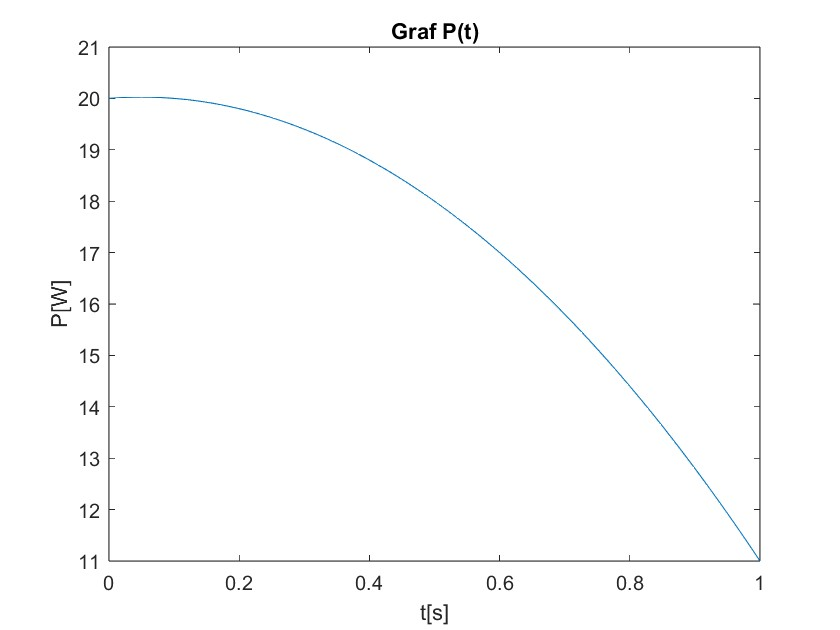
\includegraphics[width=0.9\linewidth]{Graf P(t).jpg}
    \label{P(t)}
\end{figure}
\end{frame} 

\begin{frame}
\section{Trapezna formula za integral}
\frametitle{Trapezna formula za integral}
\[
I = \sum_{i=1}^{n-1} \frac{dt}{2} \left( P(t_i) + P(t_{i+1}) \right)
\]


Rezultat funkcije \texttt{trapz} je \(17.1665\).
\end{frame}

\end{document}









